\documentclass[final,5p,times,twocolumn]{elsarticle}
\usepackage{caption}
\usepackage{amssymb}
\usepackage{amsmath}
\usepackage{multirow}
\usepackage{booktabs}
\usepackage{stfloats}
\usepackage{subcaption}
\usepackage{threeparttable}
\usepackage{graphicx}
\usepackage{array}
\usepackage{pifont}
\usepackage{tabularx}
\usepackage[hyphens]{url}
\usepackage[colorlinks,breaklinks]{hyperref}
\usepackage{tikz}
\usepackage{placeins}
\newcommand{\cmark}{\ding{51}}
\usetikzlibrary{shapes, arrows.meta, positioning, fit, calc}
\usepackage{rotating}

\begin{document}
\begin{frontmatter}

\title{DentalClaw: A Modular Workflow Platform for Standardized and Auditable Dental Imaging AI Experiments}

\begin{abstract}
\textit{Objectives:} Dental imaging artificial intelligence (AI) research requires multiple coordinated steps, including dataset preparation, quality control, model configuration, evaluation, and reproducible reporting. In practice, these tasks are often fragmented across scripts and manual procedures, creating barriers for dental researchers and clinicians. This study evaluated DentalClaw, a natural-language-driven platform that converts user intent into standardized, executable, and reviewable dental imaging workflows.\\
\textit{Methods:} DentalClaw was implemented as a modular workflow platform integrating natural-language task parsing, method selection, dataset preparation, model execution, evaluation, and structured reporting. The system was assessed on representative 2D panoramic radiograph segmentation and 3D cone-beam computed tomography (CBCT) segmentation tasks, and its intent-to-workflow decision pipeline was tested on 11 representative natural-language requests.\\
\textit{Results:} DentalClaw completed end-to-end workflows for 2D panoramic and 3D CBCT segmentation, generating standardized outputs including dataset manifests, split files, prediction results, evaluation tables, and review-oriented reports. Compared with manually assembled procedures, the platform reduced manual coordination during dataset preparation and result organization while maintaining comparable task-level performance. The intent-to-workflow evaluation achieved a weighted score of 0.977, with no incorrect workflow silently executed.\\
\textit{Conclusions:} DentalClaw demonstrated the feasibility of converting natural-language research intent into executable, auditable dental AI workflows under representative settings. The platform should be interpreted as a workflow-validation and orchestration layer rather than a new segmentation model or clinical decision-support system.\\
\textit{Clinical Significance:} By standardizing workflow execution and traceability, DentalClaw lowers the technical barrier for dental researchers while preserving a reviewable record of the data, configuration, and outputs used in AI studies.
\end{abstract}

\begin{keyword}
Dental informatics \sep Artificial intelligence \sep Digital dentistry \sep Workflow automation \sep Auditable experiments \sep Cone-beam computed tomography \sep Panoramic radiography
\end{keyword}

\end{frontmatter}

\section{Introduction}

\begin{figure*}[t]
\centering
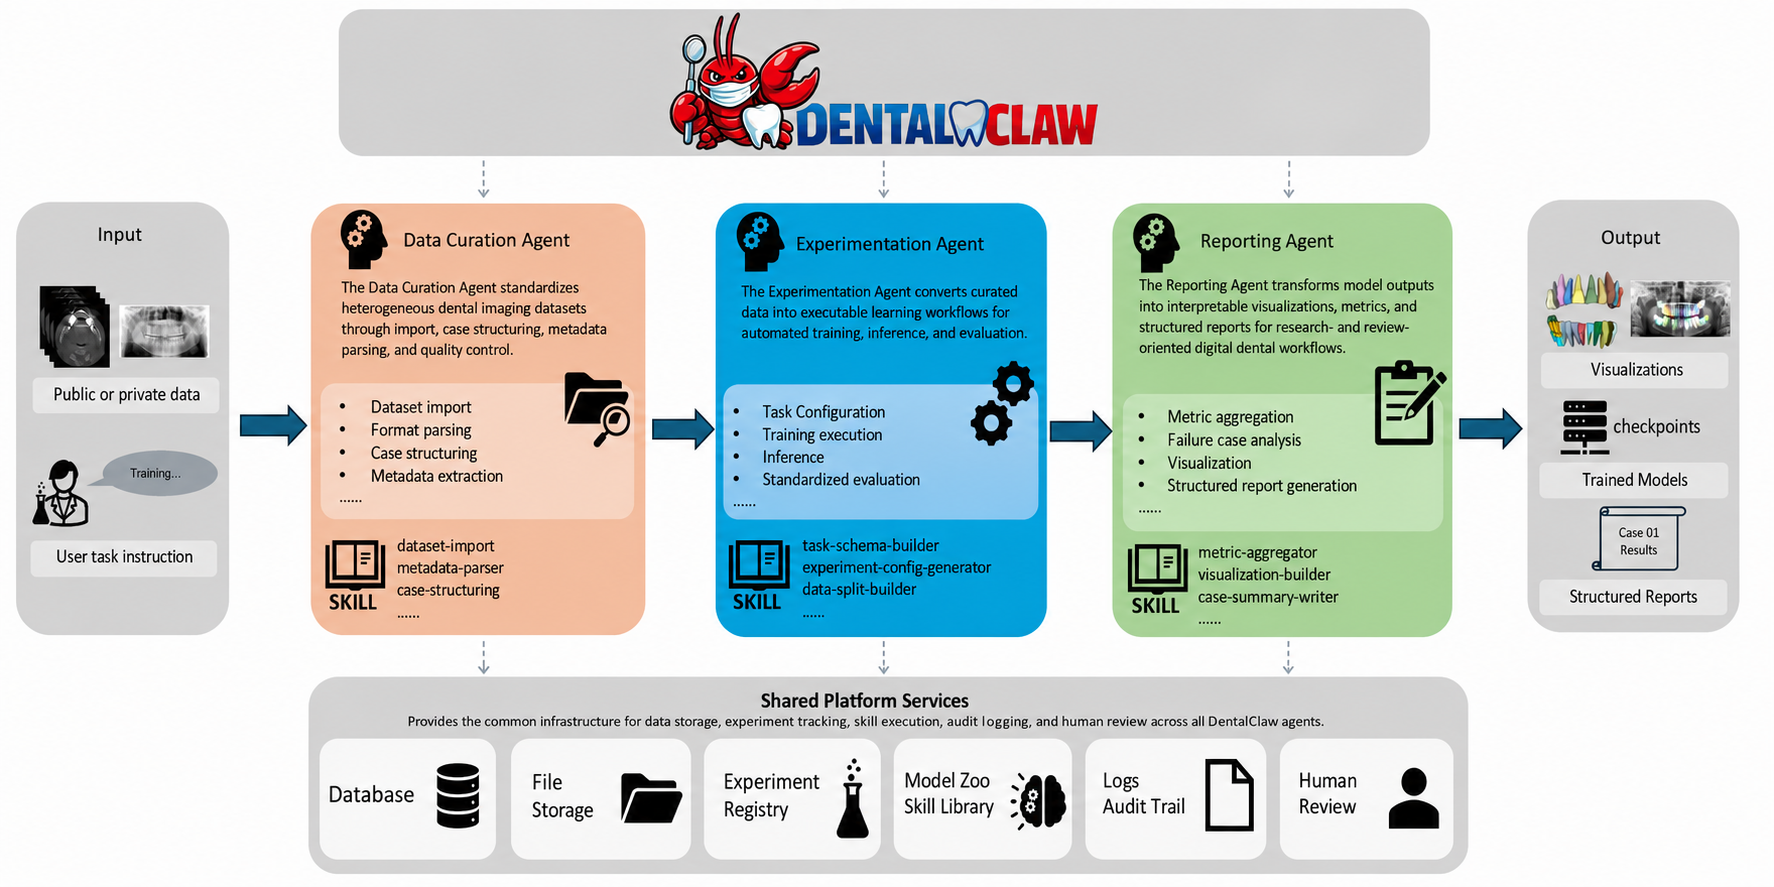
\includegraphics[width=\textwidth]{Multi-agent system architecture of DentalClaw.pdf}
\caption{Overview of the DentalClaw workflow architecture. Heterogeneous dental imaging inputs and user task instructions are processed by a central coordinator, which routes the request to dedicated data-curation, experimentation, and reporting agents. Shared platform services provide dataset management, model and skill libraries, audit logs, and human review support.}
\label{fig:system_overview}
\end{figure*}

Dental imaging AI has become increasingly relevant for tooth segmentation, lesion detection, and image-based diagnosis in digital dentistry~\cite{Horner2012,Kapila2015,Schwendicke2020,Shujaat2021}. However, translation from a research idea to a reproducible experiment remains difficult because the workflow usually spans heterogeneous data ingestion, annotation standardization, preprocessing, model configuration, evaluation, and result organization~\cite{Schwendicke2021Checklist,Polizzi2023,Dot2024DentalSegmentator}. These steps are commonly implemented as ad hoc scripts, which makes them difficult to reproduce, compare, and audit across studies.

This challenge is amplified by the heterogeneity of dental imaging data. Panoramic radiographs, CBCT volumes, and clinical annotations differ substantially in format, metadata structure, voxel spacing, and image quality. In addition, inappropriate train--test splitting or weak dataset curation may cause optimistic performance estimates and undermine reproducibility~\cite{Nemtoi2013,Schwendicke2021Checklist,Polizzi2023}. These issues create a substantial technical barrier for clinicians and dental researchers who understand the clinical problem but do not have the engineering infrastructure required to execute the complete workflow reliably.

Existing solutions partially address this problem. General medical imaging frameworks such as nnU-Net and MONAI provide powerful tools for model development and data processing~\cite{Isensee2021nnUNet,Fedorov2012Slicer}, whereas task-specific dental software tends to focus on a narrow clinical use case or a single modality. DentalClaw addresses a complementary need: it orchestrates the research workflow around the user's intent, translates natural-language instructions into candidate execution routes, and records the resulting actions in a structured and auditable form. In this sense, the platform is best understood as an orchestration layer rather than as a new segmentation model.

The objective of this study was to evaluate whether a clinician-facing workflow platform could lower the technical barrier of dental imaging AI research by converting natural-language research intent into executable, reviewable, and auditable procedures. We assessed the platform on representative 2D panoramic radiograph segmentation and 3D CBCT segmentation tasks, and we evaluated its decision pipeline on 11 representative intents spanning standard executable requests, ambiguous requests, boundary cases, and out-of-scope queries.

\begin{figure*}[b!]
\centering
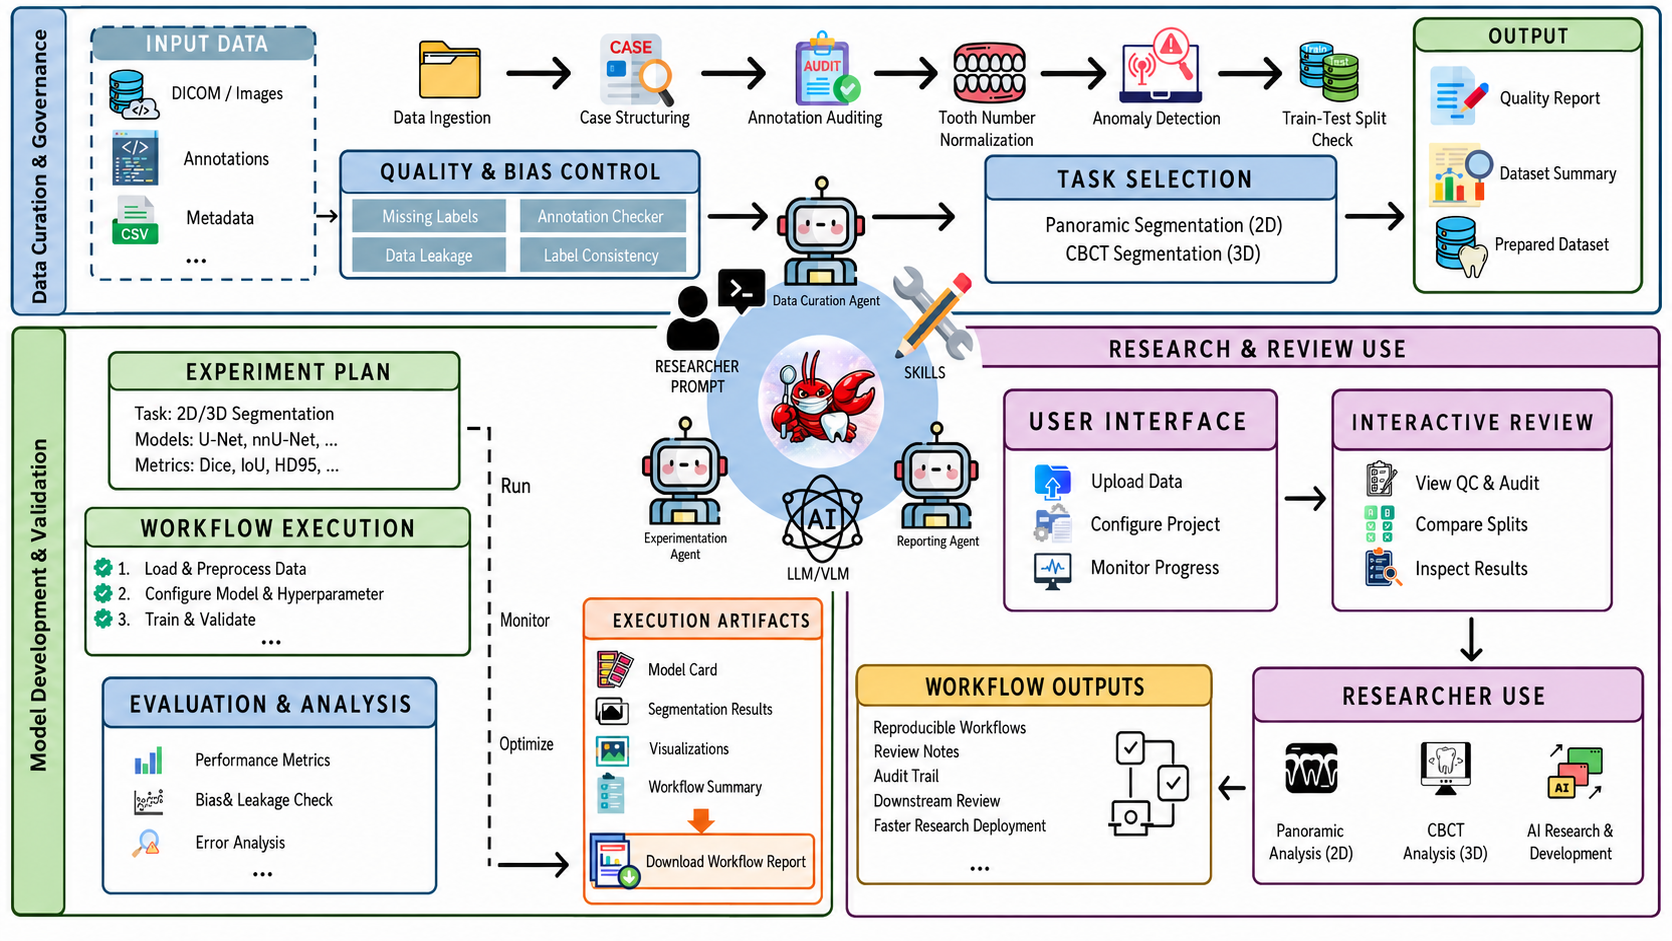
\includegraphics[width=\textwidth]{Overall workflow of DentalClaw.pdf}
\caption{Overall workflow of DentalClaw. User intent is parsed into structured fields, matched against a registry of validated methods, and routed to either an executable path or a human-reviewed external proposal. Deterministic modules perform dataset preparation, model execution, evaluation, and reporting.}
\label{fig:framework}
\end{figure*}

\section{Materials and methods}

\subsection{Study design and platform overview}
DentalClaw was implemented as a modular workflow platform built around OpenClaw~\cite{openclaw}. The system integrates a natural-language reasoning layer, an offline method registry, dataset and quality-control modules, task-specific execution routes, and structured reporting. The agent parses user intent into fields including dataset, task family, modality, mode, and optional TTA/ensemble flags. It then performs registry lookup and, when necessary, web-based proposal generation. The workflow is designed to fail safely: unsupported or ambiguous requests are rejected, and external proposals are surfaced for explicit human approval rather than being executed automatically.

The platform execution layer contains deterministic modules for dataset preparation, preprocessing, model training or inference, evaluation, and report generation. Each module records configuration, intermediate outputs, and workflow status so that the process remains auditable and reproducible. This separation of decision logic from execution logic is central to the platform design: the agent determines which workflow should be attempted, while the deterministic runner executes only the validated route or an approved external proposal.

\subsection{Datasets and representative workflows}
Two representative workflows were used for validation. The Tufts Dental Database (TDD)~\cite{panetta2022tufts} was used for 2D panoramic radiograph segmentation. After curation and audit, 968 of 1051 cases were retained for downstream processing. ToothFairy~\cite{ToothFairyDataset1,ToothFairyDataset2,ToothFairyDataset3} was used for 3D CBCT segmentation. Together, these tasks represent two common dental imaging scenarios with different dimensionality, metadata structure, and preprocessing requirements.

\subsection{Workflow execution and quality control}
All datasets were converted to a canonical case-level representation before model execution. Each case record retained image references, annotation files, modality information, and workflow status indicators. Built-in quality-control functions then checked image completeness, annotation integrity, metadata consistency, and train--test leakage risk. For flagged cases, the platform recorded the issue category and handling decision, including normalization, exclusion, or manual review.

After data validation, DentalClaw generated a task-specific execution plan specifying preprocessing rules, split assignment, output directories, and evaluation settings. The execution pipeline then invoked the relevant model route, generated predictions, computed standard segmentation metrics, and exported structured reports for review.

\subsection{Intent-to-workflow evaluation}
To test the core agent behavior, we constructed a 6-dimension weighted evaluation framework across 11 representative intents spanning standard executable requests, ambiguous queries, boundary cases, and out-of-scope requests. The intended outcome for each request was defined a priori as: whether the request was supported, whether a validated method existed, and which workflow should be selected. A decision was judged correct only if the selected route matched the intended dataset, task family, modality, and execution mode; unsupported or ambiguous requests were rejected rather than executed.

The framework included six weighted dimensions: planning, QC blocking, intent parsing, external proposal handling, ambiguity handling, and boundary identification. The platform was evaluated using the full pipeline of language detection, task parsing, literature search, registry lookup, agent decision, and method selection. Each run required approximately 50--80 s.

\section{Results}

\subsection{End-to-end workflow execution and reproducibility}
\begin{figure*}[!t]
\centering
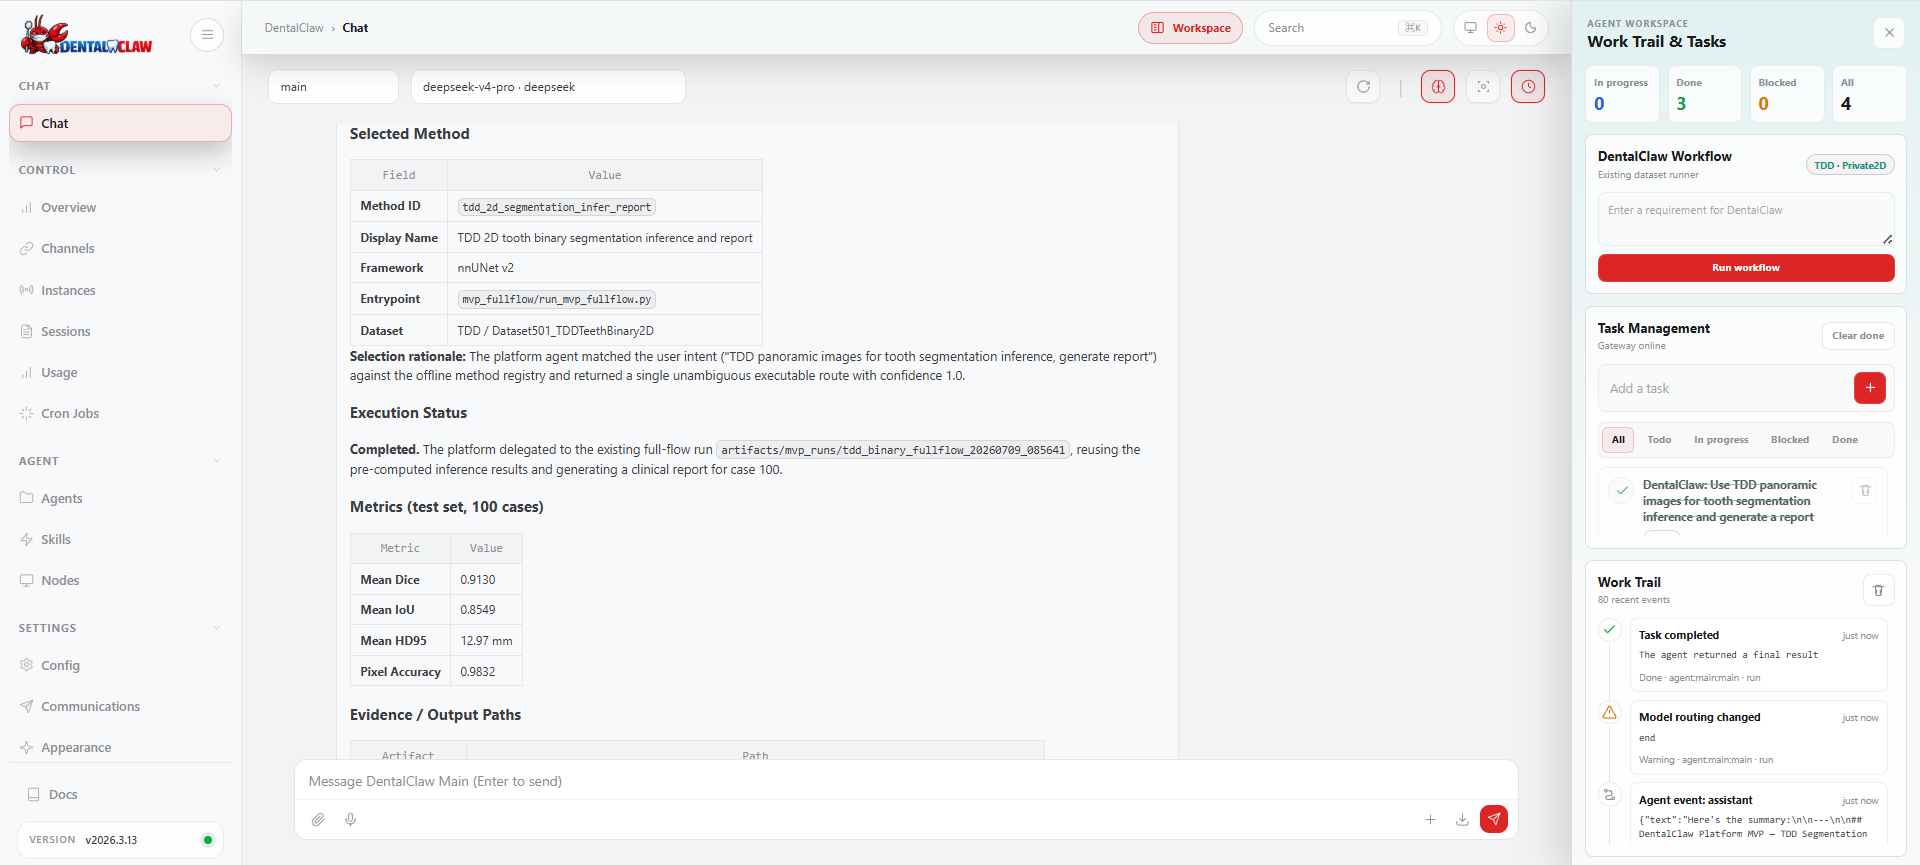
\includegraphics[width=0.95\textwidth]{Complete training.png}
\caption{Front-end workflow trace of DentalClaw showing the agent's planning, task scheduling, and report-generation state during a completed run. The interface supports human review and auditability by making the execution path visible throughout the pipeline.}
\label{fig:complete_training}
\end{figure*}

DentalClaw completed end-to-end workflows for both representative public datasets. In the 2D panoramic workflow, the platform completed dataset curation, model training, inference, evaluation, and structured reporting. In the 3D CBCT workflow, it handled volumetric data with modality-specific preprocessing, multi-model execution, and result aggregation under the same orchestration framework. Across both tasks, the platform generated standardized outputs including manifests, split files, predictions, metrics tables, and structured reports.

Table~\ref{tab:workflow_validation} summarizes the workflow-level outcomes and the comparison against manually assembled scripts. The manual baseline followed the same predefined tasks but required substantially more operator coordination. DentalClaw reduced the time spent on dataset preparation and result organization while preserving a consistent execution record for downstream review.

\begin{table*}[!t]
\centering
\small
\setlength{\tabcolsep}{4pt}
\renewcommand{\arraystretch}{1.12}
\caption{End-to-end workflow completion and coordination efficiency. The manual baseline used the same predefined workflow without additional hyperparameter tuning or model selection.}
\label{tab:workflow_validation}
\begin{threeparttable}
\begin{tabularx}{\textwidth}{>{\raggedright\arraybackslash}p{2.3cm}>{\centering\arraybackslash}p{1.6cm}>{\raggedright\arraybackslash}p{3.0cm}>{\centering\arraybackslash}p{1.4cm}>{\raggedright\arraybackslash}X>{\raggedright\arraybackslash}X}
\toprule
Task & Cases input / eligible & Main preparation findings & Completion & DentalClaw & Manual workflow \\
\midrule
Panoramic segmentation & 1051 / 968 & Missing masks; image--label mismatch & Completed & audit+prep 14 min; train 6 h 52 min; infer+eval+report 31 min; outputs: manifest, split file, predictions, metrics, report & audit+prep 3 h 26 min; train 6 h 58 min; infer+eval+organization 2 h 18 min; outputs: ad hoc logs and files \\
\addlinespace
CBCT segmentation & 63 / 43 & Metal artifacts; FOV anomalies; inconsistent volume usability & Completed & audit+prep 21 min; train 19 h 36 min; infer+eval+report 1 h 44 min; outputs: manifest, split file, volumes, metrics, report & audit+prep 6 h 12 min; train 19 h 49 min; infer+eval+organization 3 h 11 min; outputs: ad hoc logs and files \\
\bottomrule
\end{tabularx}
\end{threeparttable}
\end{table*}

\subsection{Intent-to-workflow decision accuracy}
Table~\ref{tab:intent_results} reports the decision accuracy across the 11 representative intents. The platform correctly selected the registered method for all five standard intents (1.00), correctly rejected both trap intents (1.00), and correctly handled ambiguous or incomplete requests without silently executing an incorrect workflow. For the two boundary intents involving training or detection, no registered method existed; the agent proposed external options that were flagged as \texttt{external\_suggestion} and required human review. The weighted overall score was 0.977.

\begin{table*}[!t]
\centering
\caption{Intent-to-workflow decision accuracy across 11 representative intents.}
\label{tab:intent_results}
\footnotesize
\begin{tabular}{@{}c p{5.4cm} p{2.1cm} c p{4.0cm}@{}}
\hline
\# & \textbf{Intent} & \textbf{Category} & \textbf{Score} & \textbf{Method selected} \\
\hline
1 & TDD panoramic tooth segmentation inference & standard & 1.00 & \texttt{tdd\_2d\_seg\_infer\_report} \\
2 & TDD panoramic super-resolution enhancement & standard & 1.00 & \texttt{dental\_2d\_super\_resolution} \\
3 & ToothFairy3 CBCT 3D tooth segmentation & standard & 1.00 & \texttt{toothfairy3\_3d\_seg\_...} \\
4 & Private dental data segmentation training & standard & 1.00 & \texttt{private\_2d\_segmentation\_train} \\
5 & Dental anomaly detection (panoramic) & standard & 1.00 & \texttt{dental\_anomaly\_detection} \\
6 & “Build a model with TDD” (vague task) & ambiguous & 1.00 & \texttt{platform\_clarification} \\
7 & “Write a dental AI paper” (non-CV) & trap & 1.00 & Rejected (\texttt{supported=false}) \\
8 & “Video action recognition” (non-dental) & trap & 1.00 & Rejected (\texttt{supported=false}) \\
9 & Inference on private data (no task specified) & boundary & 1.00 & \texttt{platform\_clarification} \\
10 & TDD tooth segmentation training & boundary & 0.98 & \texttt{agent\_external\_suggestion} \\
11 & TDD bbox tooth detection training & boundary & 0.98 & \texttt{agent\_external\_suggestion} \\
\hline
\multicolumn{5}{@{}c@{}}{Weighted average: \textbf{0.977} \quad (all $\ge$ 0.70 threshold)} \\
\end{tabular}
\end{table*}

These results provide evidence that the decision pipeline can distinguish executable, ambiguous, and out-of-scope requests in the tested scenarios. The platform never silently executed an incorrect workflow, and external proposals were explicitly marked for review rather than being launched without operator approval.

\section{Discussion}
DentalClaw should be interpreted as a workflow infrastructure layer rather than as a new segmentation model. MONAI and nnU-Net provide model-building primitives and automated segmentation configuration, whereas DentalClaw addresses the decision and audit problem: given a user request in natural language, which workflow should be executed, under what dataset and configuration, and with what quality-control safeguards? This separation of decision from execution is the main architectural contribution of the platform.

The results support the feasibility of this approach. DentalClaw completed representative 2D and 3D workflows, reduced manual coordination, and generated structured, review-oriented outputs. The agent decision pipeline also showed strong reliability on the tested intent set, with a weighted score of 0.977. This suggests that the platform can route a natural-language request to a supported workflow or safely reject an unsupported one without silently proceeding with an incorrect pipeline.

Several limitations remain. The evaluation was performed on representative rather than exhaustive tasks, and the current study did not include a formal usability experiment with clinicians or dental researchers. In addition, external proposals are intentionally conservative and require explicit approval before execution. This design prevents silent execution of a hallucinated or incorrect route, but it also limits automation when the task falls outside the validated registry. Future work should include broader task benchmarking, user-facing validation, and multi-backend comparisons to better quantify robustness and usability.

\section{Conclusion}
This study evaluated DentalClaw as an intent-driven workflow platform for standardized and auditable dental imaging AI research. Under representative 2D and 3D tasks, the system converted natural-language instructions into executable workflows, tracked the workflow state in a reviewable form, and generated structured outputs for dataset preparation, model execution, evaluation, and reporting. The findings support the feasibility of this workflow-oriented approach in dental imaging AI, while also clarifying that the current contribution should be interpreted as a platform validation study rather than a clinical decision-support tool or a general-purpose AI platform.

\newpage
\footnotesize
\bibliographystyle{elsarticle-num}
\bibliography{cas-refs}

\end{document}
